\begin{figure}[h!]
  \centering
  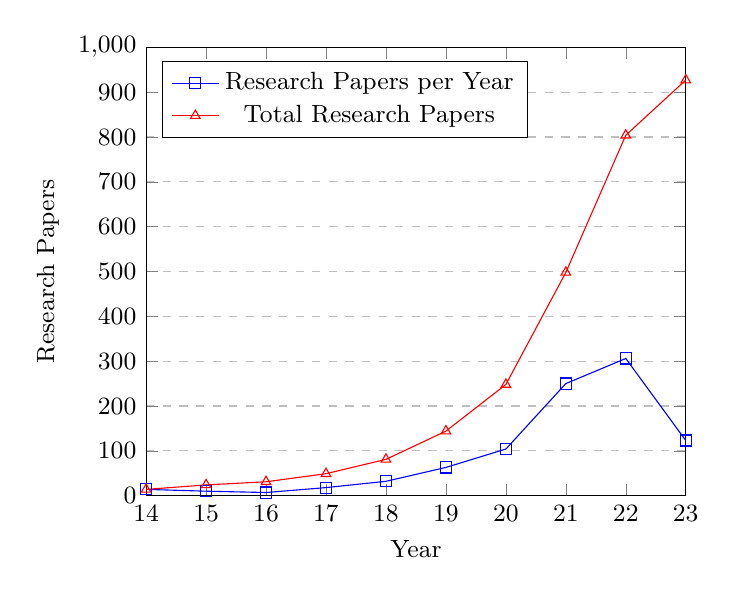
\begin{tikzpicture}
    \begin{axis}[
      title={},
      xlabel={Year},
      ylabel={Research Papers},
      xmin=2014, xmax=2023,
      ymin=0, ymax=1000,
      xtick={2014,2015,2016,2017,2018,2019,2020,2021,2022,2023},
      xticklabels={14,15,16,17,18,19,20,21,22,23},
      ytick={0,100,200,300,400,500,600,700,800,900,1000},
      legend pos=north west,
      ymajorgrids=true,
      grid style=dashed,
      tick label style={font=\small},
      label style={font=\small},
      legend style={font=\small},
    ]

      \addplot[
        color=blue,
        mark=square,
      ]
      coordinates {
        (2014,14)(2015,10)(2016,7)(2017,18)(2018,32)(2019,63)(2020,104)(2021,250)(2022,306)(2023,123)
      };
      \addlegendentry{Research Papers per Year}

      \addplot[
        color=red,
        mark=triangle,
      ]
      coordinates {
        (2014,14)(2015,24)(2016,31)(2017,49)(2018,81)(2019,144)(2020,248)(2021,498)(2022,804)(2023,927)
      };
      \addlegendentry{Total Research Papers}

    \end{axis}
  \end{tikzpicture}
  \caption{Growth of \ac{TPR} and cybersecurity related research papers found with search strategy}
  \label{fig:research_papers_growth}
\end{figure}
